\documentclass{article}
\usepackage{color}
\usepackage{tikz}
\usepackage{float}
\usepackage{tabularx}
\usepackage{amsmath}
\usepackage{amssymb}
\usepackage{listings}
\usepackage{enumitem}
\usepackage{syntax}
\usepackage{csquotes}
\usepackage{pgfplots}
\usepackage{parskip}
\usepackage{fancyhdr}
\usepackage{vmargin}
\usepackage[backend=biber]{biblatex}
\addbibresource{references.bib}


\definecolor{dkgreen}{rgb}{0,0.6,0}
\definecolor{gray}{rgb}{0.5,0.5,0.5}
\definecolor{mauve}{rgb}{0.58,0,0.82}


\lstset{frame=tb,
  numbers=left,
  stepnumber=1,
  language=Java,
  aboveskip=3mm,
  belowskip=3mm,
  showstringspaces=false,
  columns=flexible,
  basicstyle={\small\ttfamily},
  numberstyle=\color{gray},
  keywordstyle=\color{blue},
  commentstyle=\color{dkgreen},
  stringstyle=\color{mauve},
  breaklines=true,
  breakatwhitespace=true,
  tabsize=2,
  moredelim=**[is][\color{red}]{@}{@},
}

\setlength{\grammarindent}{12em}

%\renewcommand{\lstlistingname}{Algorithm}
%\newcommand{\tablerow}[4]{ #1 & #2 & #3 & #4\\}
\newcommand{\n}[0]{\\[\baselineskip]}

%
% #1 - Module code
\newcommand{\maketitlepage}[2]{
\begin{titlepage}
	\centering
    
\includegraphics[scale = 0.4]{01-standard-vertical-black.png}\\	% University Logo
	\textsc{\LARGE #1}\\[0.5 cm]				% Course Code
	\rule{\linewidth}{0.2 mm} \\[0.4 cm]
	{ \huge \bfseries \thetitle}
	\rule{\linewidth}{0.2 mm} \\[0.5 cm]
	\textsc{\large \thedate}\\[1.5 cm]
	
	\begin{minipage}{0.4\textwidth}
		\begin{flushleft} \large
			\emph{Lecturer:}\\
			#2
			\end{flushleft}
			\end{minipage}~
			\begin{minipage}{0.4\textwidth}
            
			\begin{flushright} \large
			\emph{Submitted By:} \\
			\theauthor
		\end{flushright}
        
	\end{minipage}\\[2 cm]
	
\end{titlepage}
}

\title{Predicting energy use of appliances}
\author{140011146}

\makeatletter
\let\thetitle\@title
\let\theauthor\@author
\let\thedate\@date
\makeatother

\begin{document}


\maketitlepage{CS5014 Machine Learning}{David Harris-Birtill\\Kasim Terzi\'{c}}


\section{Introduction}
A paper \cite{paper} on prediction models of energy use of appliances using data gathered from a low energy house presented different prediction models to try and gain an understanding of appliance use in buildings. 
\n
As a machine learning exercise, the same raw dataset is taken and used to create a regression model. Each step of the machine learning methodology is carefully followed and documented to show off different consequences of decisions made. The resulting models are evaluated against test data and the results are discussed to see why a simple linear model is not a strong fit for the dataset.


\section{Data preprocessing}
The data preprocessing steps are first written in the python notebook as an example to show how that particular step works. Afterwords, before the start of choosing and training models, the preprocessing steps are written again as extensions to \texttt{sklearn}'s pipelines. This makes for a modular design as each step of the preprocessing process can be included or changed in the pipeline if tweaking is needed.
\subsection{Splitting test set}
Before even looking at the data, the first thing that was done was to split the data into training and test data. The test data will be put away until the end to run our different models on. This is to represent new unseen data, therefore we do not want to inspect at all so we can test how well our model performs against new data. This is why this splitting into test data is the very first thing that is done. The first decision is to decide the percentage split of training and test data. The percentage chosen represents a trade off between less training or less testing data.
\n
One disadvantage of splitting the data into training and test sets before looking at its contents is the risk of introducing sampling bias\cite{geron}. This is because the test set may not be representative of our dataset as the sampling is done completely randomly without taking into account different proportions of feature values. This may be fine on a larger dataset, but as our dataset is relatively small, it is a trade off we make for ensuring we don't introduce bias in our models from looking at the test data. Additionally, a validation set is not split again from the training data. This is done to keep all data for training due to the smaller dataset we have. Any parameter tuning or cross validation done is therefore done all on the training data. To counter the disadvantage of not having the separate validation set, k-fold cross validation is used.


\subsection{Data visualisation}

\subsubsection{Histograms}
We can visualise the data by plotting histograms of each column. This will tell us some information about how the data for each feature is distributed, and whether there might be errors in the data.

\begin{figure}[H]
\centering
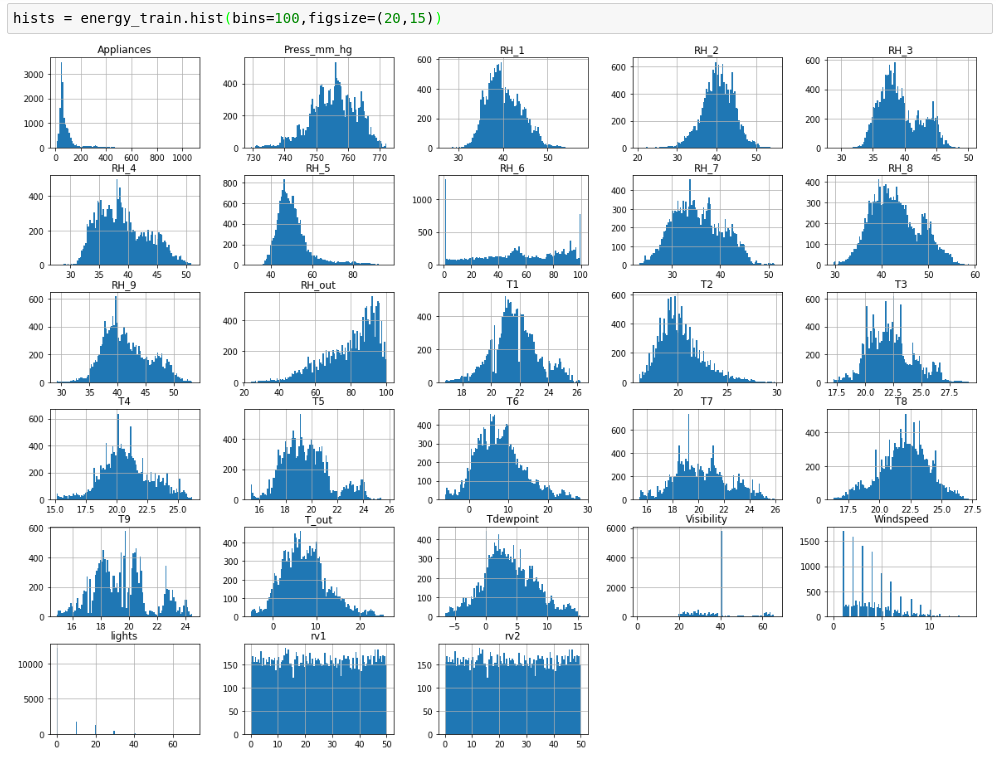
\includegraphics[width=1\textwidth, keepaspectratio]{imgs/histograms.png}
\caption{Histograms of all data features except for time.}
\end{figure}
\noindent
Time is not plotted here as we have not converted it from its string form yet. However, we expect the time to be quite regular, as the data is gathered as measurements after every certain timestamp over a period of 137 days. 
\n
We can see from the histograms, many of the temperature and relative humidity values follow a relatively normal distribution. Some features have very discrete values, for example the \textit{lights} feature only has a few unique values. There are also some features that don't follow a normal distribution. For example, the histogram for \textit{RH\_6} is interesting as it as many values at the extreme ends of the histogram. This is different from most of the other humidity sensors but can be explained because this is the one humidity sensor that was placed in the exterior of the house. Another example of an odd histogram is the \textit{Visibility}, as one value dominates compared to all others. Though this can be explained as the visibility being normal for most measurements and only changes rarely, it may not make for a good input feature as its values do not change very much.

\begin{figure}[H]
\centering
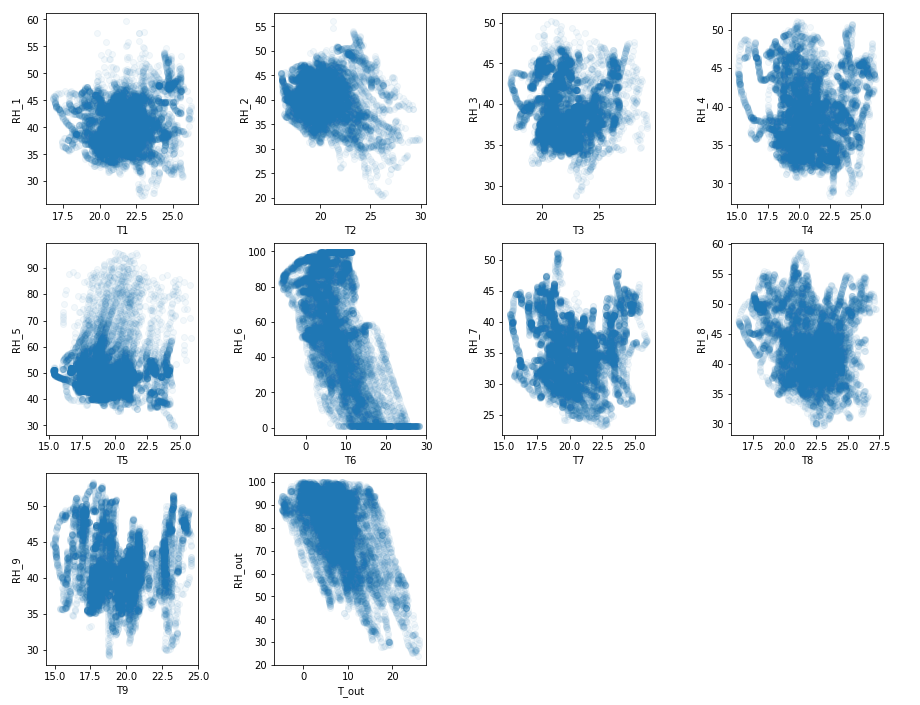
\includegraphics[width=1\textwidth, keepaspectratio]{imgs/t-rh-correlation.png}
\caption{Plotting each temperature measurement against the humidity of the same sensor to see if there is any correlation between the two.}
\end{figure}
\noindent
We can also see that temperatures and humidity sensors are not correlated to each other well, this shows they are not redundant features and may both be important in the prediction. 


\subsection{Data cleaning}
To clean the data, we must first observe what kind of data is given. From \cite{paper}, we know our data describes temperatures, relative humidity, energy consumption, pressure, windspeed, visibility and time. From knowledge of what the data represents, we can clean any values that don't make sense, for example negative humidity or extreme temperatures.
\n
From our visualisation, we can see in the histograms that there are no nonsensical values in our dataset, however, we cannot be sure this also applies to our unseen test data, so we should still include the cleaning step in our methodology, even if nothing is cleaned initially. Additionally, we can see there are no NaN or missing values from looking at the \texttt{pandas} dataframe, but we should still include a step for cleaning these values in case the test data has such values. 

\subsection{Converting datetime}
One column of the given data is a string timestamp, which includes the date and time the measurement was taken. 
\begin{lstlisting}[caption={Example timestamp snippet}, backgroundcolor = \color{lightgray}]
2016-01-26 12:30:00
\end{lstlisting}
In \cite{paper}, the time was converted into 3 input features: Number of seconds from midnight (NSM), Week status and Day of the week. The week status and day of the week were categorical features while number of seconds is numerical. However, these kind of features do not take into account the cyclical nature of time.
\n
To keep the cyclical nature of time, a different approach was used where the time of day and day of week features were created using a sine and cosine transform \cite{cyclic}. The use of the trigonometric functions keep the cyclical features, so for example 5 seconds before and after midnight would be represented as being 10 seconds apart rather than one being 5 seconds and the other being 86395 seconds. The sine and cosine features must be used together, as just using one of the two features gives a 12-hour representation rather than a full 24-hour representation. 



\subsection{Feature selection}
Now that we have prepared the inputs and converted the timestamp, we must choose a suitable subset of features of training. It is important to choose a strong features that help give better accuracy while removing unimportant features that may hurt the performance of the model. It is also better to have fewer features to keep the model simpler. It may help to improve the accuracy of some models and reduces computational requirements. Further, it would be easier to explain and understand a simple model compared to a very complex one. 
\n
The correlation between all features can be computed and visualised. The correlation is mapped to its absolute value, since negative correlation is just as strong as positive correlation only in the opposite direction. This lets us see if any pair of features are very strongly correlated and one could therefore be removed as it would be redundant. As we are wanting to use a linear model to begin with, the correlation between the input features and the output is important as that is how new output values will be predicted. Unfortunately, though many of the features correlate with each other, most have quite weak correlations with the output.

\begin{figure}[H]
\centering
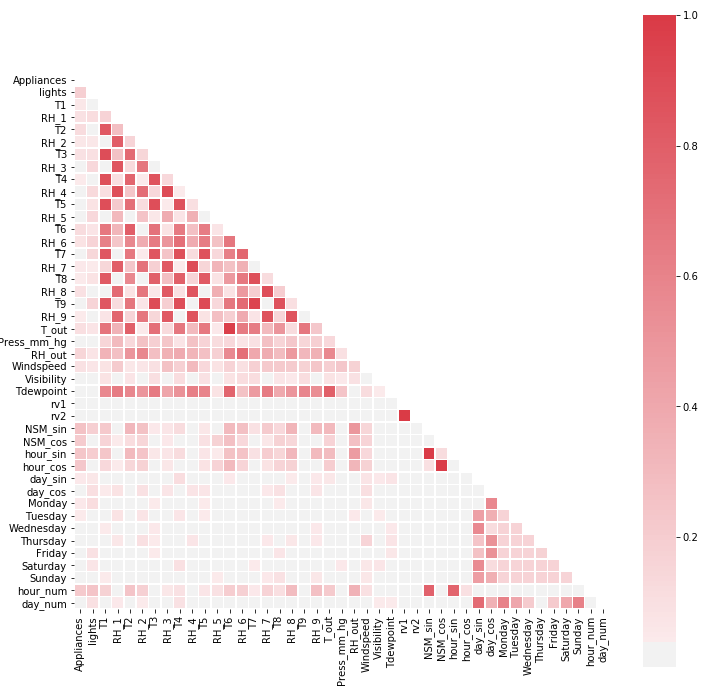
\includegraphics[width=1\textwidth, keepaspectratio]{imgs/all-corr.png}
\caption{Correlation matrix of all features in our dataset}
\end{figure}
\noindent
From the correlation matrix, it is clear the random variables do not correlate to any of the other features - including the output feature - except each other, so it would be important to remove them from our list of input features. Further, temperature readings seem to be correlated to themselves. For example, T1 is most well correlated to other temperature readings. This does make sense as most of the temperature readings are all from inside the house, so they would be expected to be quite similar to each other. Compared to other input values, all the temperature features are also most similar to other temperatures, giving them higher correlation among themselves. 

\subsubsection{Choosing date/time feature}
To choose which form to convert the timestamp to be, the correlation between each time feature and the output ``Appliances" features can also be computed. 
\begin{figure}[H]
\centering
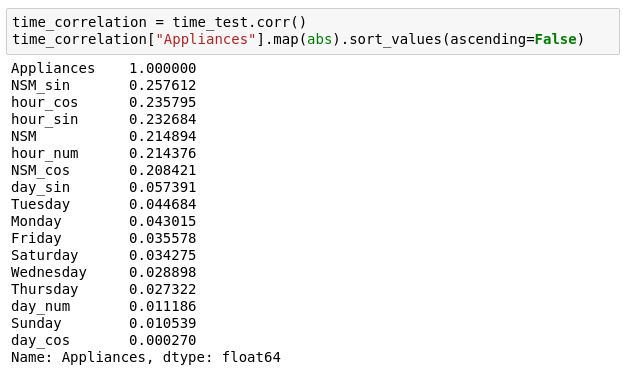
\includegraphics[width=0.7\textwidth, keepaspectratio]{imgs/time-correlation.png}
\caption{Correlation of different time input features against the output feature.}
\end{figure}
\noindent
We can see that the time of the day is a strong feature compared to the day of the week.  \texttt{hour\_sin} and \texttt{hour\_cos} was chosen as their correlation is better than \texttt{NSM} and \texttt{hour\_num}. They were chosen over \texttt{NSM\_sin} and \texttt{NSM\_cos} as \texttt{NSM\_cos} has a lower correlation but must be included if \texttt{NSM\_sin} is chosen. Our correlation matrix also shows that the cyclic \texttt{NSM} and cyclic hour values correlate strongly to each other, so only one of the two should be chosen as the other is redundant. 
\n
For the day of the week feature, we should again choose just one to avoid redundancy. The sine transformation of the day of the week is the most correlated to the output feature, however the cosine transform is not. Because of the consistency of the categorical features, it is chosen over the cyclical day of the week. 

\subsubsection{Feature selection algorithms}
To choose the features we could simply set a threshold on the correlation of each input feature against the output and remove all features below the threshold. A more systematic way would be with methods like univariate tests.
\n
We shall choose to use two different methods. The first is the simple way of removing features under a threshold. The threshold is chosen as the correlation of the random variables. The reasoning behind this is that as the random variables are just completely random variables which have very low correlation to the output, any input features with \textit{less} correlation than that should not be used. Further, we shall use the \texttt{KBest} selector from \texttt{sklearn} as our second method for feature selection. This was chosen to contrast the simple threshold removal. From looking at our correlation matrix, there are very little features that the random variable threshold would remove. This would leave us with a large set of input features. For contrast, we can select fewer features to keep using k best selection and compare how these two selection methods may impact performance of our models. There are two options for a scoring function for the k best selector: \texttt{f\_regression} and \texttt{mutual\_information}. Mutual information was not selected as it estimates the mutual information of a continuous target variable, but not all our input features are continuous. 

\section{Model selection, training and results}
For the process of model selection, we first select a simple linear regression model. We test on both methods of feature selection. The error values from training come from cross validating the trained model on the training data.
\n
After each model, the error is checked and a graph of the predicted values and true values is plotted to understand the reason behind the performance of the models.

\subsection{Model performance}
In general, the errors and results obtained had a similar performance to the results from \cite{paper}. Despite the different aspects to the input feature preprocessing and our feature selection choosing a smaller reduced set of features, our linear models were not able to improve much past the paper's results. 

\subsubsection{Linear regression}
First, we start with the simplest model of linear regression. 
\begin{figure}[H]
\centering
\begin{tabular}{| c | c | c |}
\hline
\textbf{Score} &  \textbf{Threshold feature selection} & \textbf{KBest feature selection (k=10)} \\
\hline
RMSE & 92.57 & 94.86 \\
\hline
\textbf{$R^{2}$} & 0.198 & 0.16 \\
\hline
\end{tabular}
\caption{Error values after cross validation for a linear regression model.}
\end{figure}
\noindent
We see that our models get very similar errors to the given paper. Using the simple threshold feature selection seems to perform better while the KBest features performs just slightly worse, though the difference is small such that it could be due to variance in the data. The errors from the paper sit between our two models, with an \textsc{rmse} of 93.21 and an $R^{2}$ of 0.18. 
\n
We are also able to reproduce the residual plot from the paper, which shows why linear regression is not a strong model for this dataset. The residuals show that when the true output value increases, the error in our model also increases. This also suggests there may be some missing variables as a predictive pattern is leaked as a residual\cite{residual}.
\begin{figure}[H]
\centering
\begin{minipage}{0.45\textwidth}
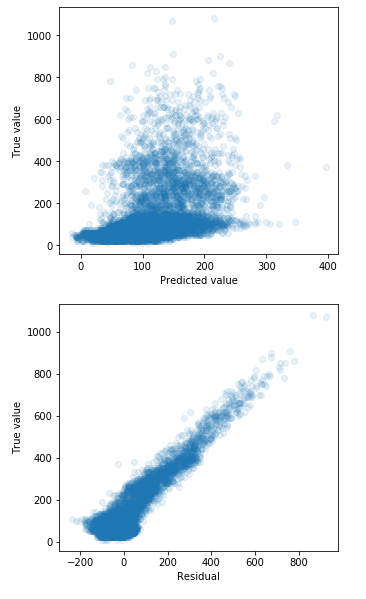
\includegraphics[width=1\textwidth, keepaspectratio]{imgs/linreg-simple.png}
\end{minipage}
%
\begin{minipage}{0.45\textwidth}
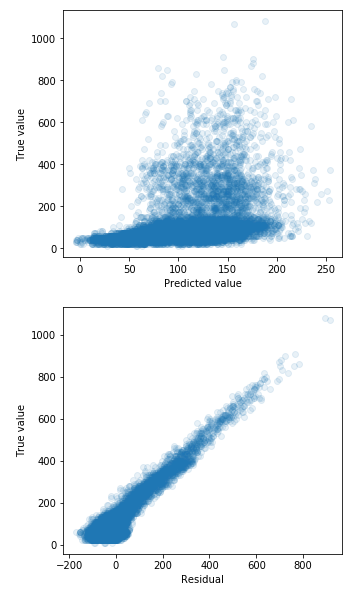
\includegraphics[width=1\textwidth, keepaspectratio]{imgs/linreg-kbest.png}
\end{minipage}
\caption{Predicted value and residual graphs of the two linear regression models. The model with simple feature selection is on the left and the model with KBest (k=10) feature selection is on the right.}
\end{figure}
\noindent
Because our model is underfitting, it may not help to add regularisation in the form of ridge or lasso regression. Suppressing our features with a regularisation parameter would do little to improve performance. Perhaps if we increase the complexity of our model with polynomial features, we may be able to find out more. 

\subsubsection{Polynomial regression}
As our first linear model does not seem to fit the data well, we can try using basis expansion with polynomial expansion to increase the variance of the model. 
\begin{figure}[H]
\centering
\begin{tabular}{| c | c | c |}
\hline
\textbf{Score} &  \textbf{Threshold feature selection} & \textbf{KBest feature selection (k=10)} \\
\hline
RMSE & 84.43 & 91.77 \\
\hline
\textbf{$R^{2}$} & 0.33 & 0.21 \\
\hline
\end{tabular}
\caption{Error values after cross validation for a polynomial regression model of degree 2.}
\end{figure}
\noindent
With polynomial expansion of degree 2, we are able to reduce our errors, but our models are still performing poorly. The residual pattern still occurs as expected. Particular to note is using KBest selection seems to hurt our model, as the polynomial KBest model is unable to get errors lower than that of the linear model with the simple threshold selection. However, the different is relatively small, especially given that there are more than 10 more features in the threshold selection models. 
\n
Furthermore, we see that in all our models, we are still predicting output values that are negative. This doesn't make sense in the context of our dataset and problem because the power consumption of appliances cannot be negative. This further suggests that a linear model may not be suitable for this dataset as getting negative values is an inherent characteristic of a linear model. 
\begin{figure}[H]
\centering
\begin{minipage}{0.45\textwidth}
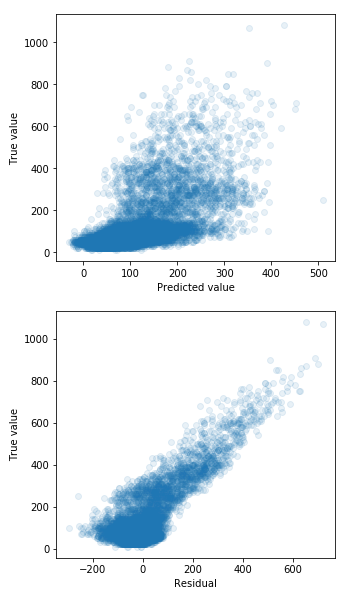
\includegraphics[width=1\textwidth, keepaspectratio]{imgs/poly-simple.png}
\end{minipage}
%
\begin{minipage}{0.45\textwidth}
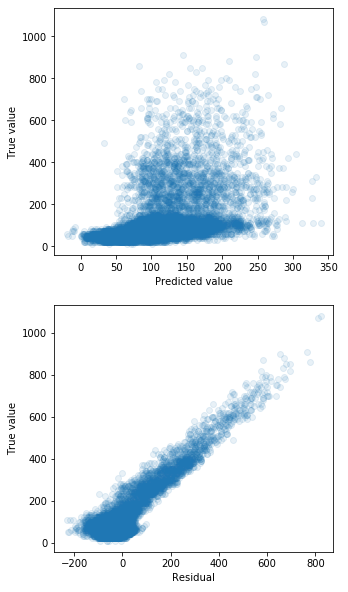
\includegraphics[width=1\textwidth, keepaspectratio]{imgs/poly-kfold.png}
\end{minipage}
\caption{Predicted value and residual graphs of the polynomial models. The model with simple feature selection is on the left and the model with KBest (k=10) feature selection on the right.}
\end{figure}
\noindent
From here, it would be a good to try different regression models like support vector machines or random forest. However, due to a lack of understanding for how these different models work and a lack of time, their application as been omitted. 

\section{Results and evaluation}
After having trained our few models against the training data and getting some error statistics, we can finally use our testing data to see how well the models work. Due to us using no validation set and running cross-validation on our training data, it would be expected that the errors on the testing data are slightly higher. 
\n
As our simple feature selector performed better in both the simple linear and polynomial model, we shall use that as our testing feature selection. The result was very similar to the result of the models run during validation so there is little more insight that can be provided. 


\section{Discussion}
The approach taken was careful to ensure no looking at the test data and little bias where possible. Some trade offs were taken, such as not having a validation set in an attempt to save more data for training and not looking at the whole dataset before splitting the training and test sets to prevent sampling bias. By using the pipeline structures provided by \texttt{sklearn}, each step of the machine learning process could be set modularly and clearly. This also ensures that the test data goes through the exact same preprocessing steps as the training data did.
\n
After moving from simple linear to polynomial regression with two different sets of input features, it was found that none of the models resulted in good performance on the dataset. From the graphs of the predicted values, we can see because we are using an underlying linear model, there are predicted values which are negative. The characteristic of linear models for not restricting the output from negative values, shows it is not very suitable for this dataset. Further, the residual graphs show that as the actual value increases, the error increases as well, meaning there could be missing variables. 
\n
Given more time and understanding, more regression models that are not linear could have been used and evaluated to see how they perform in contrast. The paper the dataset comes from seemed to have better success with other models, though their error values for test data was still relatively high. Perhaps this dataset could be viewed as a classification problem instead of a regression problem, where appliance energy consumption can be grouped into ranges of values. A look at the value counts of the dataset show most output values lie in discrete values between 0 to 200 (eg, 30,40,50...) so a different viewpoint would make an interesting comparison.


\printbibliography

\end{document}



